\section{Sensor Overview}
\label{sec:overview}

We explore using a new class of RGB-D sensor such as the Creative Senz3D~\cite{nguyen2015vietnamese} to build 3D mesh models of plant leafs. The sensor contains a high resolution color camera ($1280 \times 720$ pixels) adjacent and parallel to a lower resolution depth camera ($320\times240$ pixels).  A flash IR emitter adjacent to these cameras illuminates the scene and depth sensor measures the time-of-travel for the reflected light as well as its reflectance over its pixel grid.  These modalities are illustrated in Figure~\ref{fig:plantnoise}.  Our approach is to leverage of the strengths of each modality to compensate for weaknesses in the other.  

In order to gain the most from the sensors, we model effects due to sensor alignment and sensor noise.  Pose alignment between the color and depth cameras as well as intrinsic parameters are calibrated using Zhang's method~\cite{Zhang2000}.  This is possible for the depth camera since it also returns an IR reflectance at each pixel, and the checker board can be detected in this.  In the rest of this section the occlusion effects of displaced sensors are modeled and the depth noise is modeled.


\subsection{Occlusion Modeling}

The color camera is offset to the side of the depth camera, and so at depth discontinuities, such as leaf boundaries, some pixels visible by the depth camera may be occluded in the color camera.  During mesh fitting these occluded pixels may project into the leaf mesh and result in large depth distortions.  In~\cite{Alenya2011} an interpolated z buffer is used to detect these occluded pixels.  Here we present a visibility analysis method that is closer to the stereo occlusion modeling~\cite{Belhumeur1996}.  We do not require rectification as there is no pixel matching, but we use the known horizontal offset of the color camera from the depth camera.

A row of pixels in the depth camera are projected out into world coordinates, as illustrated in Fig.~\ref{fig:occlusion}.  Then using just the planar position of the color camera (and not its orientation), the angle to the color sensor, $\theta(i)$, can be calculated for each depth pixel $i$.  Starting from the left-most pixel we incrementally step through all the pixels and set $\theta_{\max}(i) = \max(\theta(i),\theta_{\max}(i-1))$.  This keeps track of the largest angle seen so far in the row traversal.  Occluded pixels are then simply:
\beq
\theta(i) < \theta_{\max}(i). \label{eq:occluded}
\eeq
This assumes occluding objects are wide enough not to be seen around.  Results of this are shown in Fig.~\ref{fig:beanimageprocess}($b$).  The only filtering done on this is to remove single occluded pixels with no neighbors as these occlusion labels are likely to be due to noise.

\begin{figure}
\begin{center}
   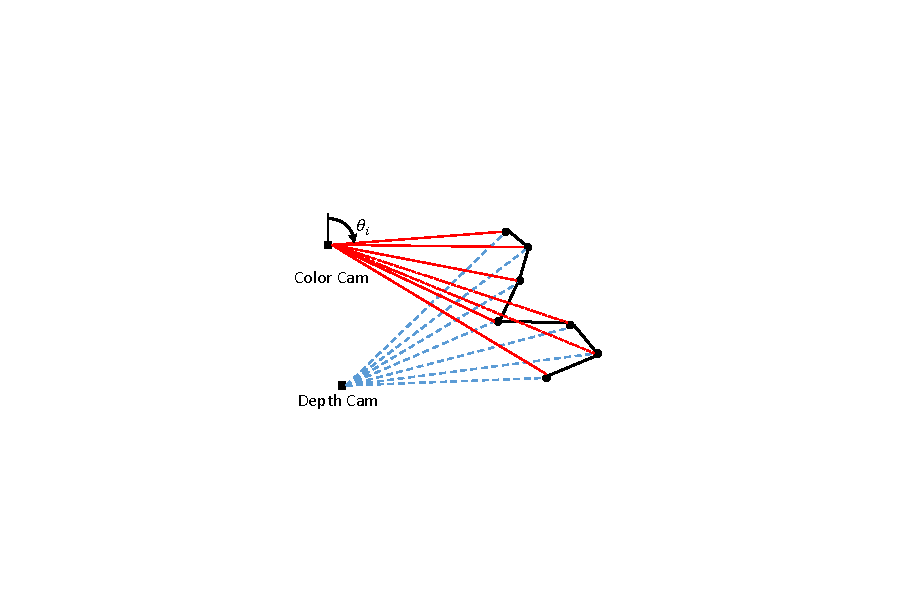
\includegraphics[trim=130 90 140 90,clip,width=0.75\linewidth]{Figures/OcclusionModeling}
\end{center}
   \caption{Occlusion modeling }
\label{fig:occlusion}
\end{figure}


\subsection{Noise Characterization}
\label{sec:noise}

Depth measurements are performed along pixel rays, and hence depth noise is modeled as a one dimensional random variable, $\varepsilon$, along the ray for each pixel along its ray direction.  We observe significant noise correlation between sequential measurements of a given pixel, and so do not assume sequential measurements are independent.  On the other hand averaging multiple measurements reduces the noise.  To capture partial correlation we propose the following simple noise model. 

The depth noise, $\varepsilon$, is modeled as the sum of an image-varying term, $\varepsilon_I$, and a scene-varying term, $\varepsilon_S$:
\begin{equation}
\varepsilon = \varepsilon_I + \varepsilon_S. \label{eq:epsilon}
\end{equation}
The term $\varepsilon_I$ models the random change in depth for camera pixels of subsequent images of a static scene from a static camera.  To quantify this term we measured the standard deviation $\sigma_I$ in depth of each pixel for a batch of 300 images of a fixed scene containing a flat matte surface.  We repeated this at different poses and depths, and with different surface albedos.  While target depth, inclination, albedo, and pixel position are all correlated with $\sigma_I$, we found that the best predictor for $\sigma_I$ was the IR reflectance intensity, as shown in Figure~\ref{fig:sigmainterframe}.  For typical scenes the single measurement noise in depth is roughly 5mm, although for low reflectivity objects or objects at long range this noise can increase significantly.  Fortunately plant leafs are good IR reflectors.

\begin{figure}
\begin{center}
   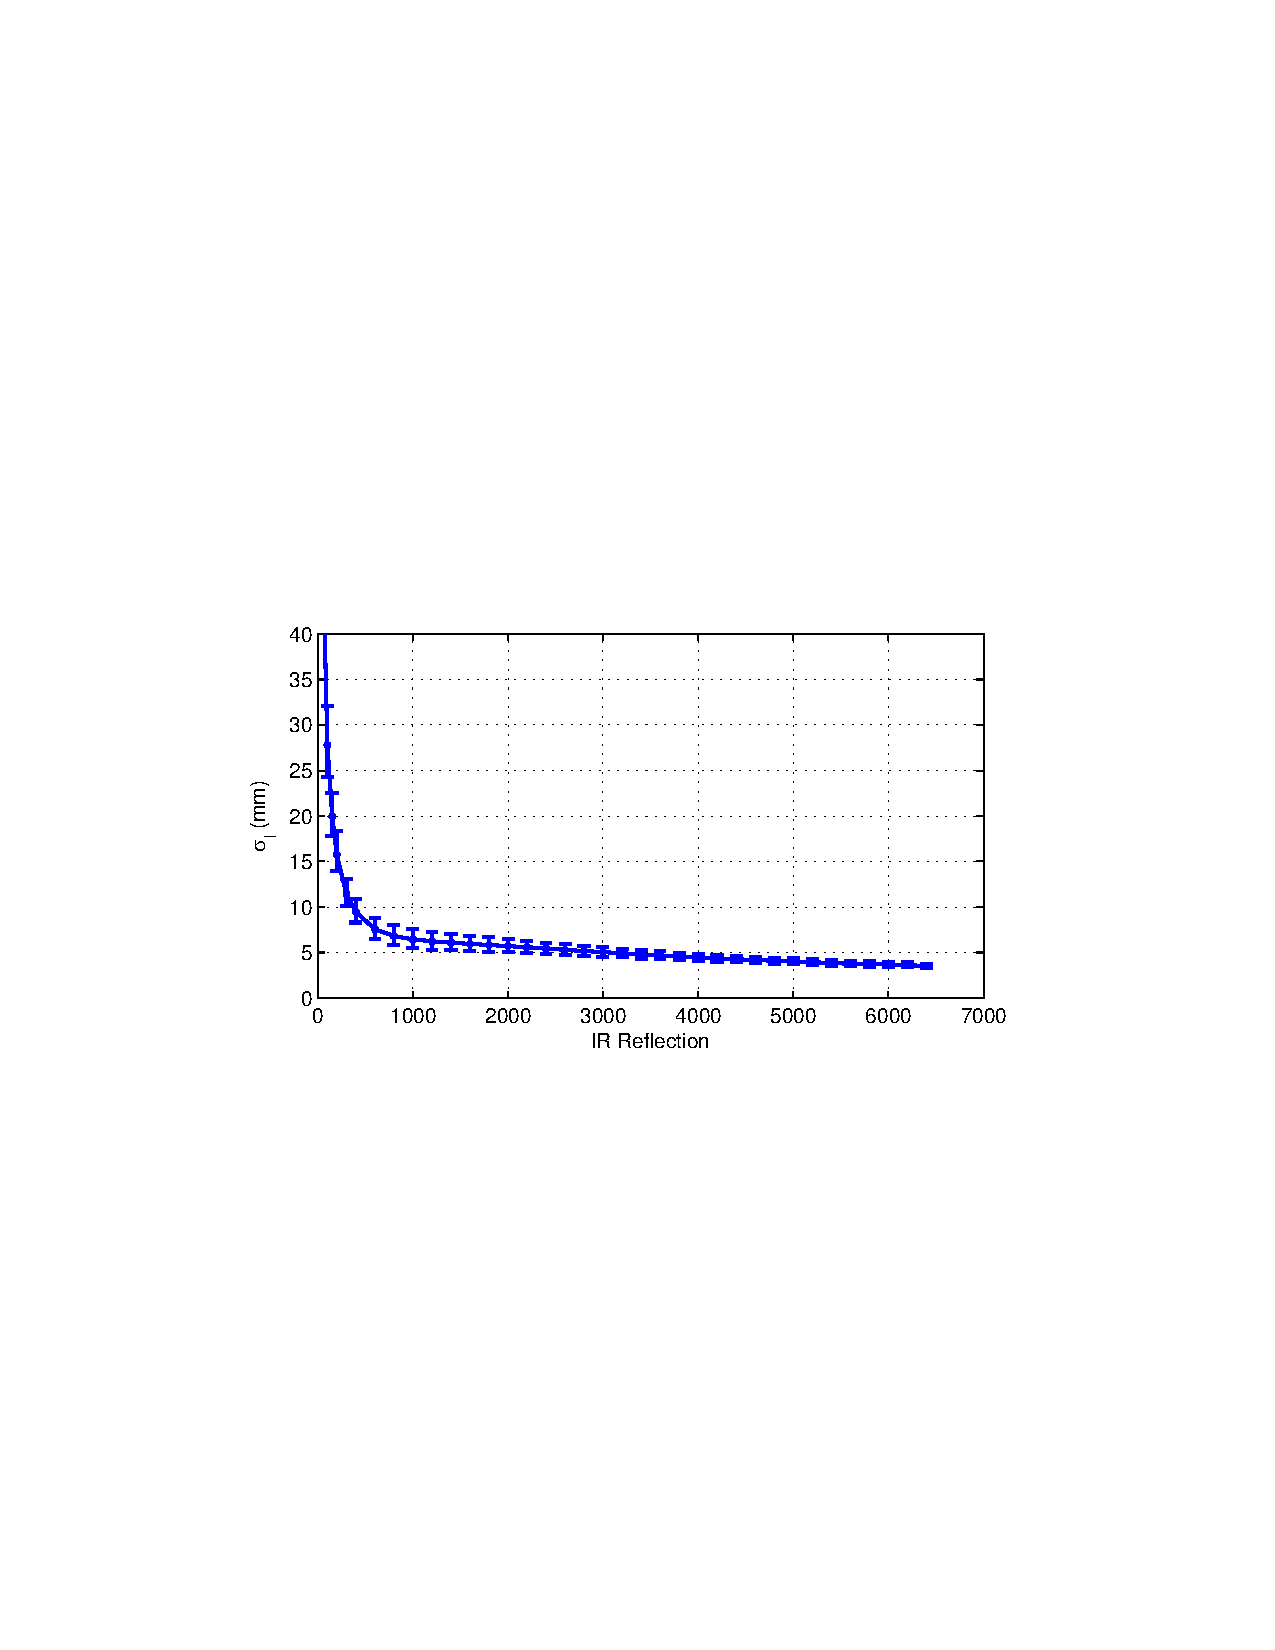
\includegraphics[trim=120 280 110 290,clip,width=0.9\linewidth]{Figures/SigmaInterframe}
\end{center}
   \caption{Image-varying noise, $\sigma_I$, is predicted well by the IR reflectance in raw units returned by the camera, see Figure~\ref{fig:plantnoise}($b$).  The scene-varying noise, $\sigma_S$, is plotted for comparison.}
\label{fig:sigmainterframe}
\end{figure}

Averaging depth measurements of a fixed scene will reduce the noise from $\varepsilon_I$, but will not reduce the noise from $\varepsilon_S$.  This latter scene-varying term is constant for a static scene, but changes when the scene changes.  To characterize this noise we first eliminated (approximately) the image-varying noise contribution by averaging over a large number of images (300).  Then assuming $\varepsilon_S$ is independent and identically distributed between pixels, we measured the variance of the pixel depth errors between a known flat surface and the estimated surface.  In our experiments we obtained $\sigma_S=6.5mm$, and found that it was insensitive to changes in depth.

The total pixel noise can be estimated assuming independence of $\varepsilon_I$ and $\varepsilon_S$, and is given by:
\begin{equation}
\sigma^2 = \frac{\sigma_I^2}{N} + \sigma_S^2,\label{eq:sigma}
\end{equation}
where $N$ is the number of images averaged over.  When averaging 5 or more depth images the scene-varying contribution, $\sigma_S^2$, will dominate.  There are additional sources of noise not modeled by this.  These include object specularities, and mixed-depth pixels on object edges.  These tend to produce very large image-varying noise, $\sigma_I$, and we can filter these points by discarding depth pixels with $\sigma_I>20$mm.  


\begin{figure}
\begin{center}
\begin{tabular}{cc}
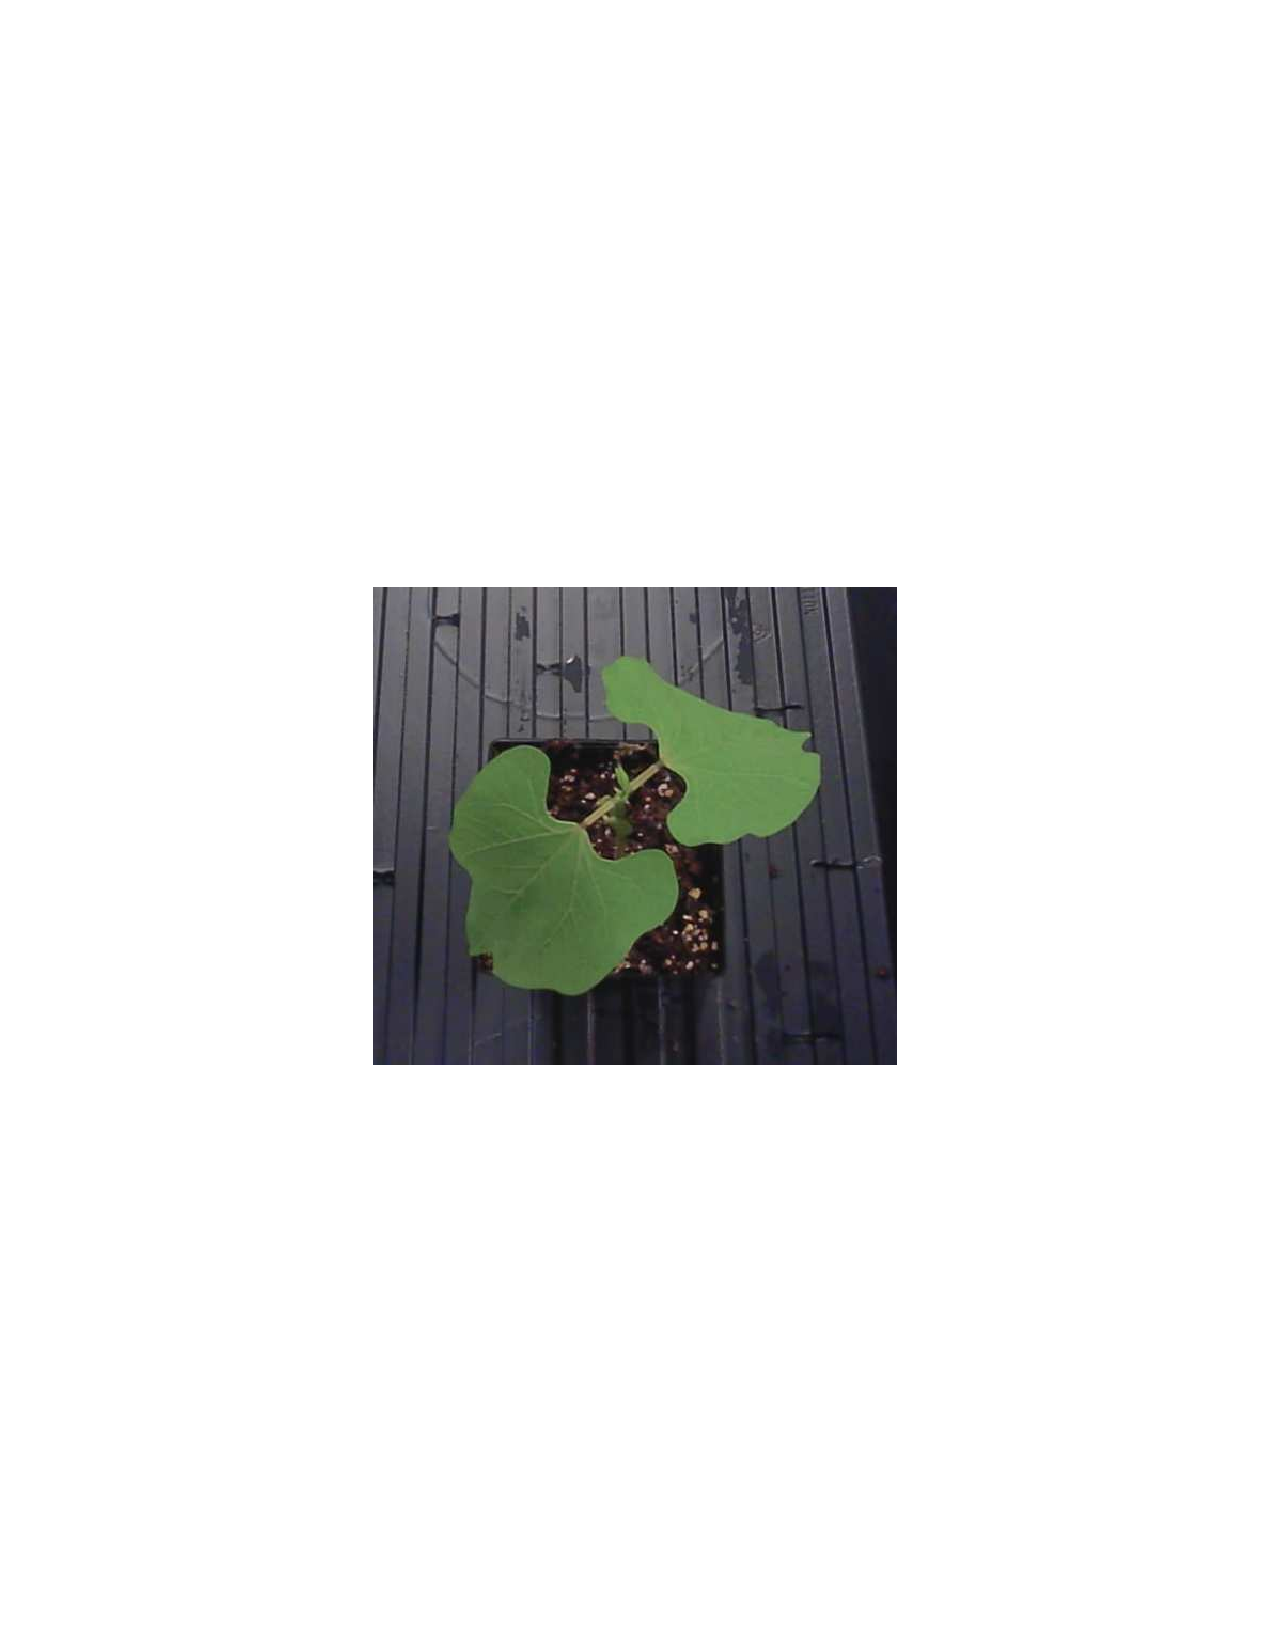
\includegraphics[trim=190 280 190 290,clip,width=0.47\linewidth]{Figures/beanColor} &
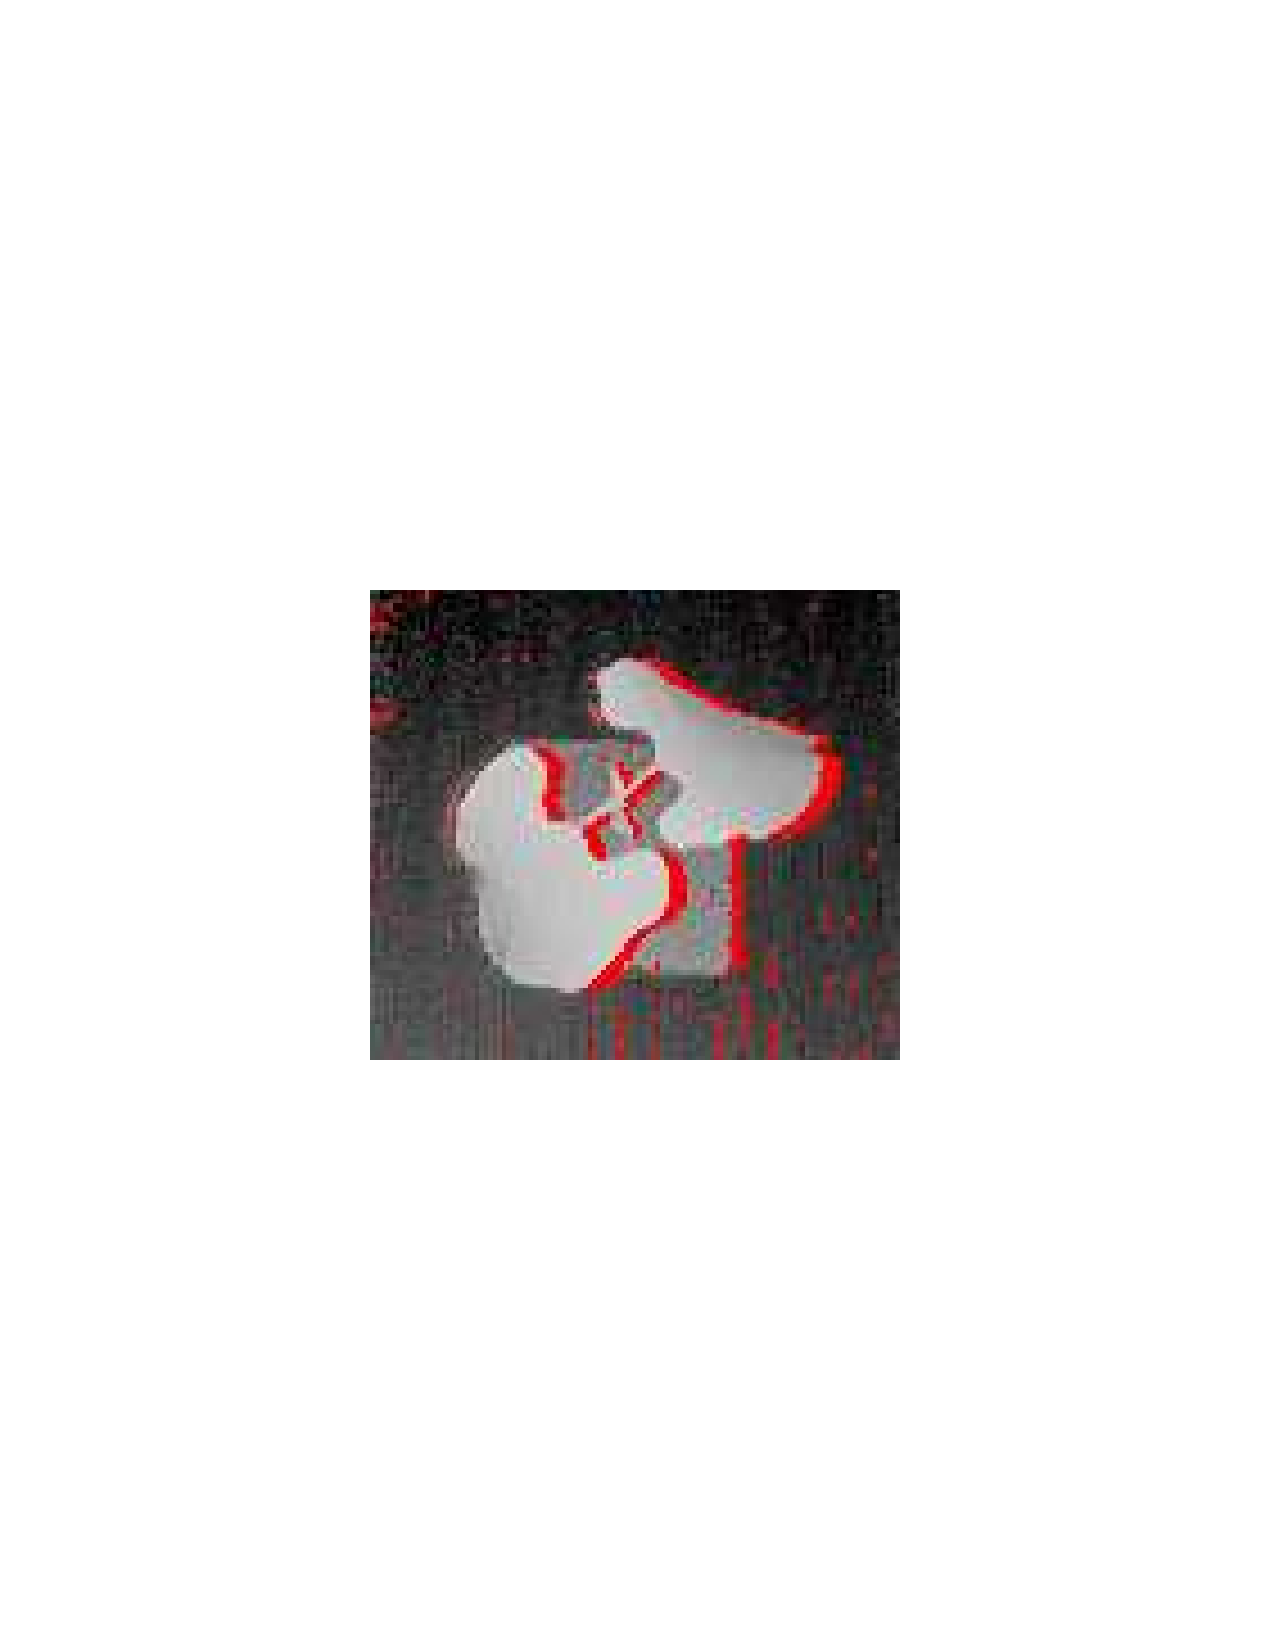
\includegraphics[trim=190 280 190 290,clip,width=0.47\linewidth]{Figures/beanDepth} \\
($a$) & ($b$) \\
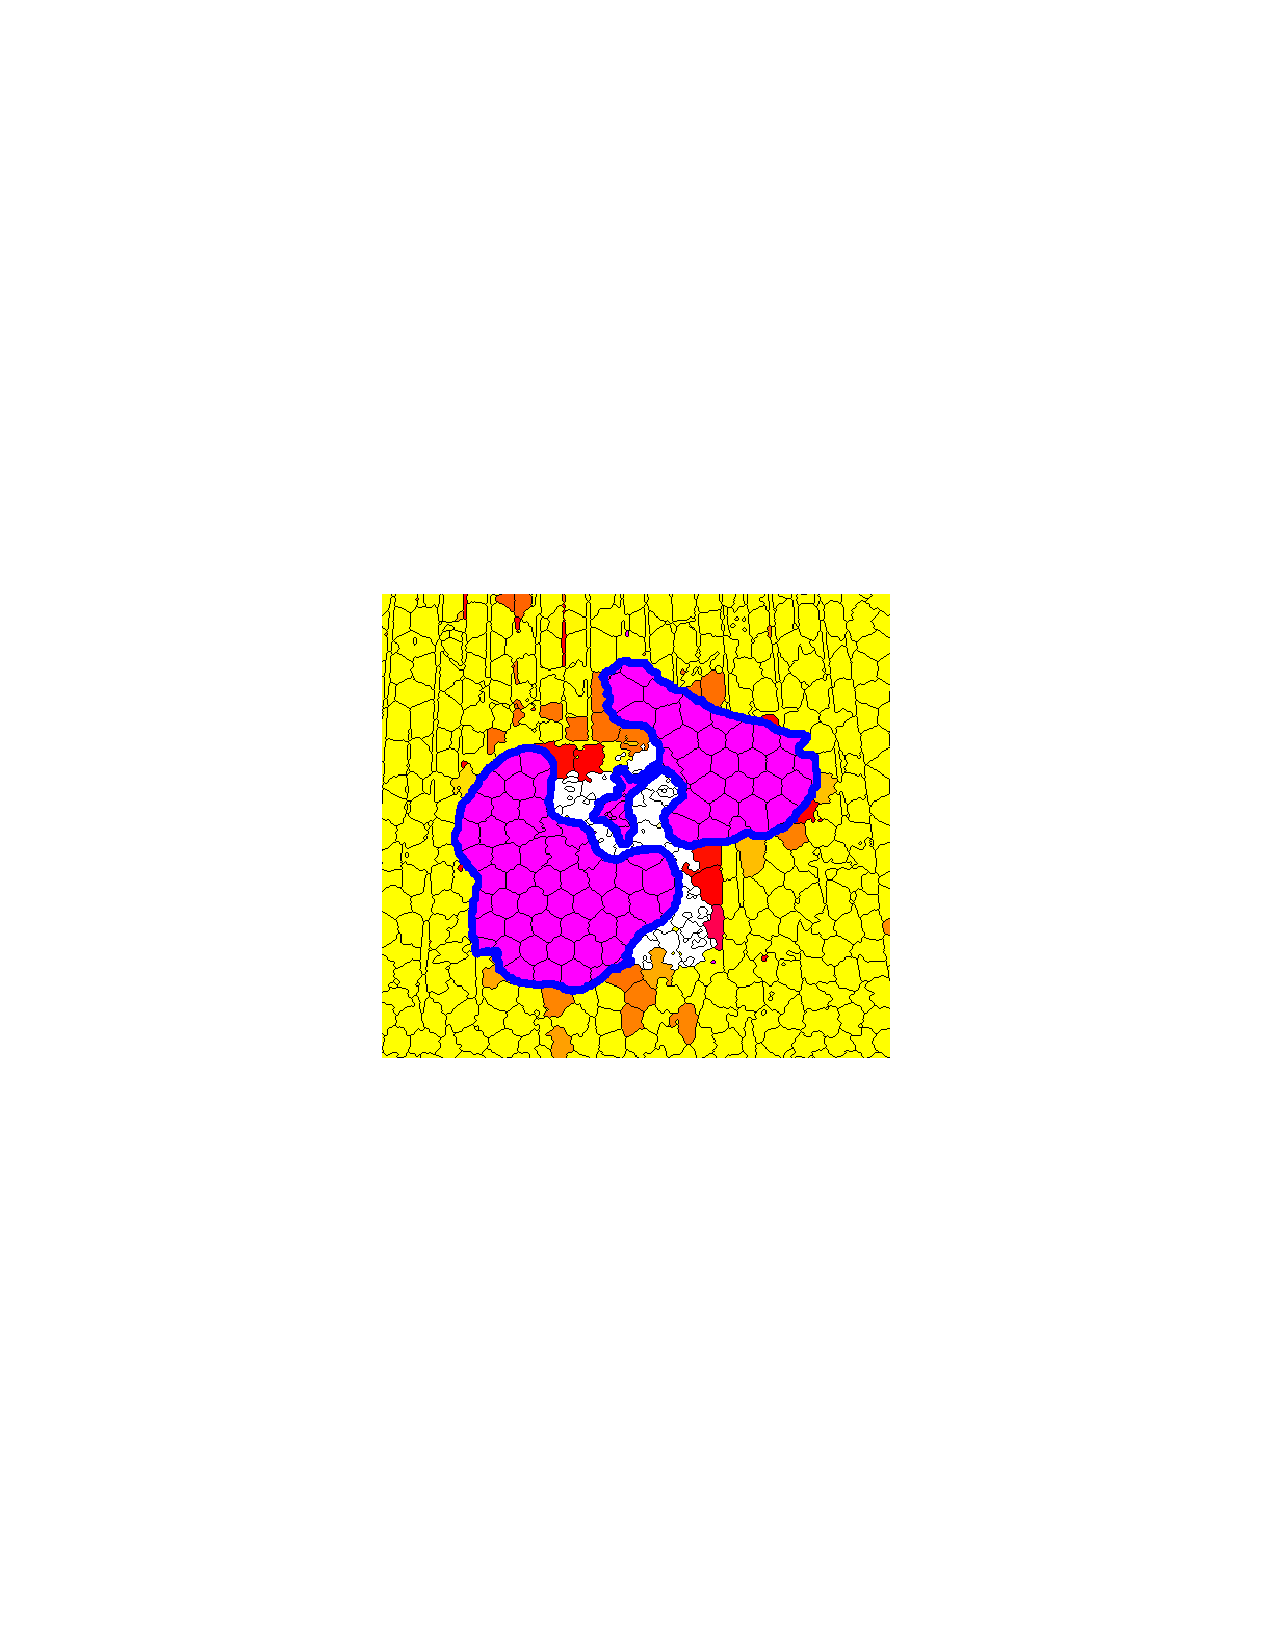
\includegraphics[trim=190 280 190 290,clip,width=0.47\linewidth]{Figures/slic_cropped2} &
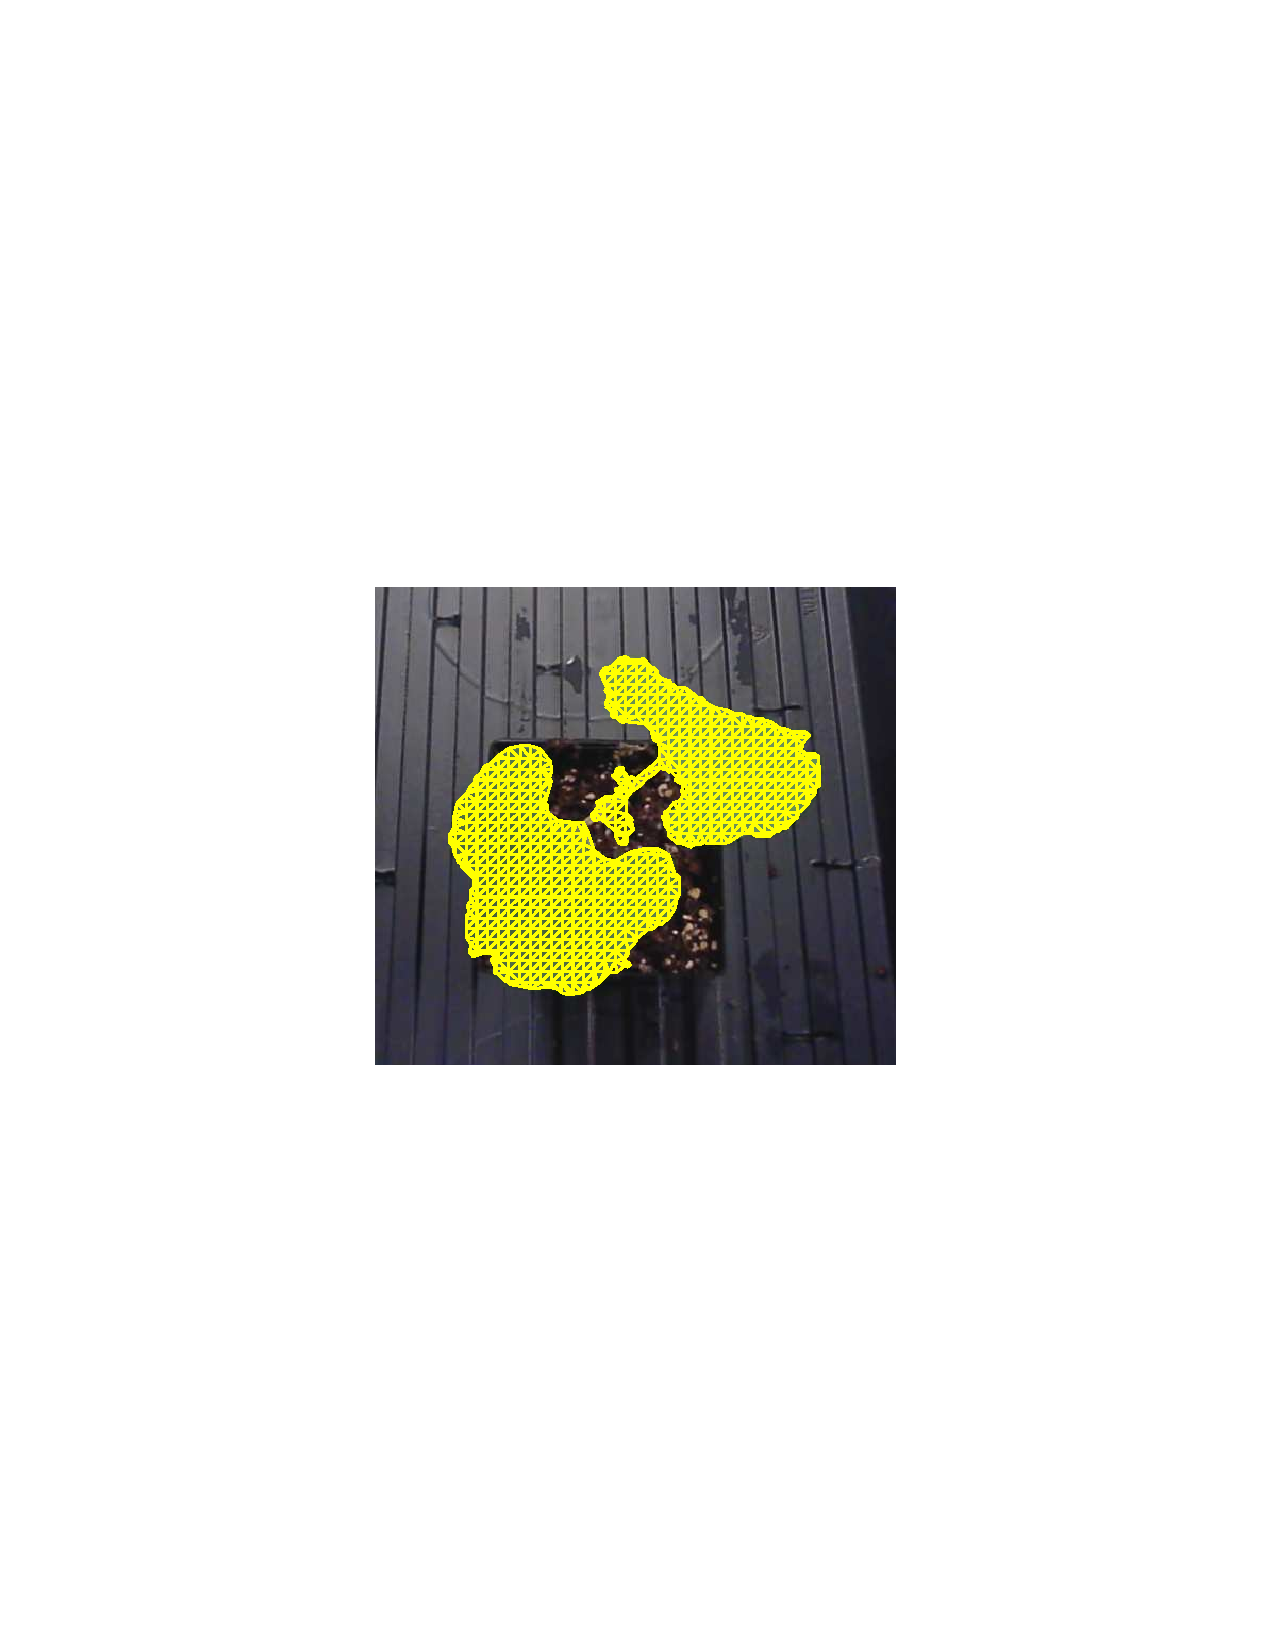
\includegraphics[trim=190 280 190 290,clip,width=0.47\linewidth]{Figures/beanColorMesh} \\
($c$) & ($d$) \\
\end{tabular}
\end{center}
\caption{Initial algorithm steps.  ($a$) Color image portion on plant.  ($b$) Depth image, where red pixels are those that are masked out using the method in Fig.~\ref{fig:occlusion} as they are not visible in the color image. ($c$) SLIC superpixels on LAB color space.Each of the superpixels are colored with the mean L, a and b values of that particular superpixel. The leaf boundaries obtained by integrating the superpixels having the leaf pigments are shown in green dots. ($d$) An mesh is defined in the color image with evenly spaced vertices within and along the leaf boundaries. }
\label{fig:beanimageprocess}
\end{figure}

